\section{Results}
Results and discussion.
\input graphsize

\input csc2f_table

\begin{figure}[htbp]
	\vspace{-2pt}
	\begin{center}
		       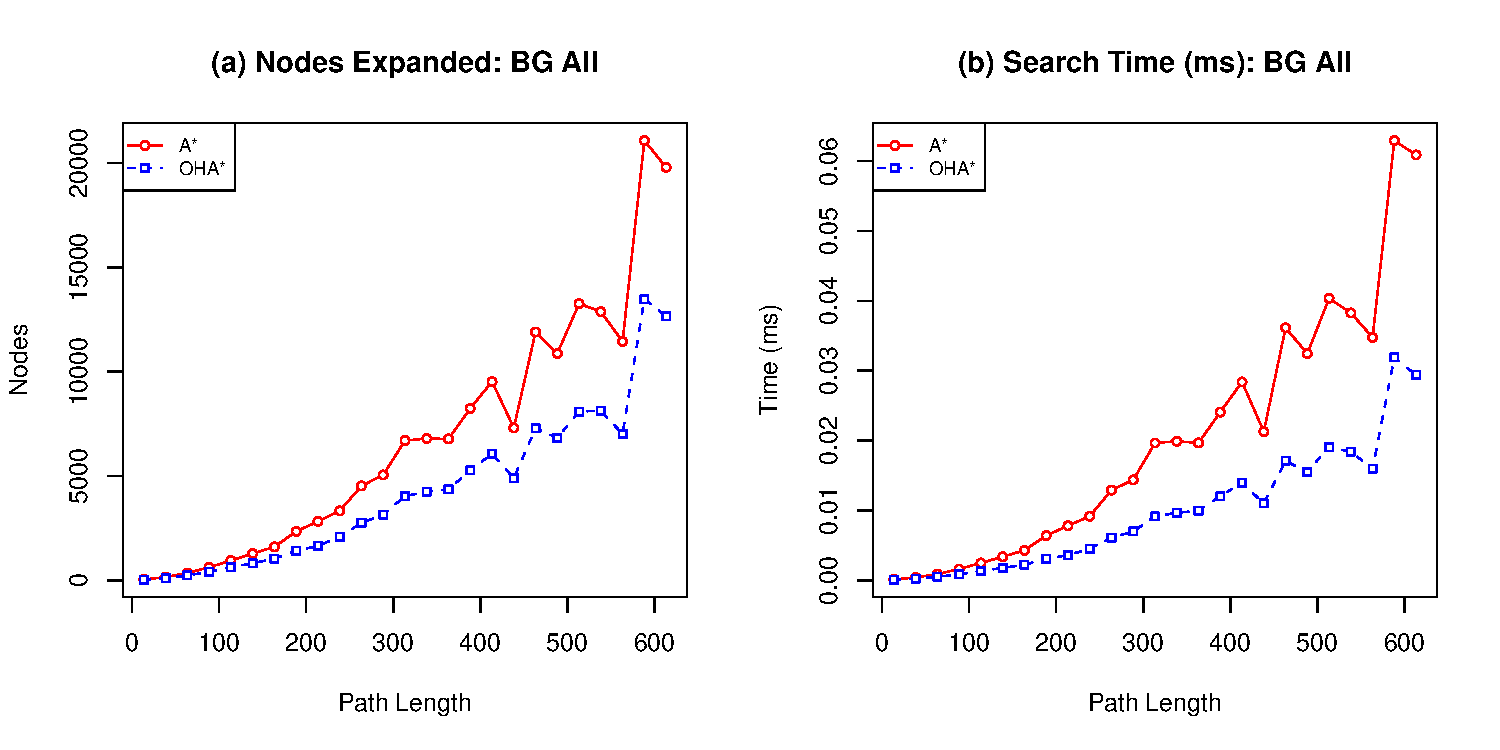
\includegraphics[scale=0.35, trim = 20mm 17mm 20mm 5mm]{diagrams/bg_effort.pdf}
	\end{center}
	\caption{Average number of nodes expanded across all maps in the Baldur's Gate set.}
	\label{aha-fig:pathquality}
	%\vspace{-12pt}
\end{figure}
\par \indent


\begin{enumerate}
 \item{Nodes expanded and nodes touched}
 \item{Example of our method vs A*? probably earlier, in overview section?}
 \item{Search time}
 \item{Graph size; can we put all 4 together???}
 \item{things that can affect performance; clustering approach, obstacles. 
	The point is still the same -- there is less to gain when only small
	clusters can be created. 
	We explore this issue empirically on the map from Example 1 by creating 4 distinct
	variants, each one containing a greater number of randomly placed obstacles
	ranging from 10\% to 50\%. 
	As before, we randomly generate 100 distinct experiments for each variant and evaluate
	the performance of both algorithms. 
	Figure 10 presents the average number of nodes expanded with respect to path length. 
	The performance of the algorithm will degrade in these cases; in the worst
	case every traversable node is a cluster and the performance of the algorithm is
	identical to A*. }
\end{enumerate}
